\subsection{Normalisierung}
\label{sec:Normalisierung}

Quelle: DatabaseCamp \cite{normalisierung}

\paragraph{1. Normalform} Eine Relation liegt in der ersten Normalform vor, wenn alle Attributwerte \hl{atomar} vorliegen.

Das bedeutet, dass \hl{jedes Datenfeld lediglich einen Wert enthalten darf}. Außerdem sollte sichergestellt sein, dass jede Spalte nur Werte desselben Datentyps (Numerisch, Text, etc.) enthält. Folgende Beispiele müssten entsprechend verändert werden, damit eine Datenbank in der 1. Normalform vorhanden ist:

\begin{multicols}{2}
	\begin{itemize}
		\item Adresse: “Hauptstraße 1, 12345 Berlin” 
		\begin{itemize}
			\item Straße: “Hauptstraße” 
			\item Hausnummer: “1”
			\item PLZ: “12345”
			\item Ort: “Berlin”
		\end{itemize}
		\columnbreak
		\item Rechnungsbetrag: “128,45 €”
		\begin{itemize}
			\item Betrag: “128,45”
			\item Währung: “€”
			\vfill
		\end{itemize}
	\end{itemize}
\end{multicols}

\paragraph{2. Normalform} Eine Relation liegt in der zweiten Normalform vor, wenn sie in der ersten Normalform vorliegt und alle \hl{Nichtschlüsselattribute voll funktional vom gesamten Primärschlüssel abhängig} sind.


\begin{wrapfigure}{r}{0.55\textwidth}
	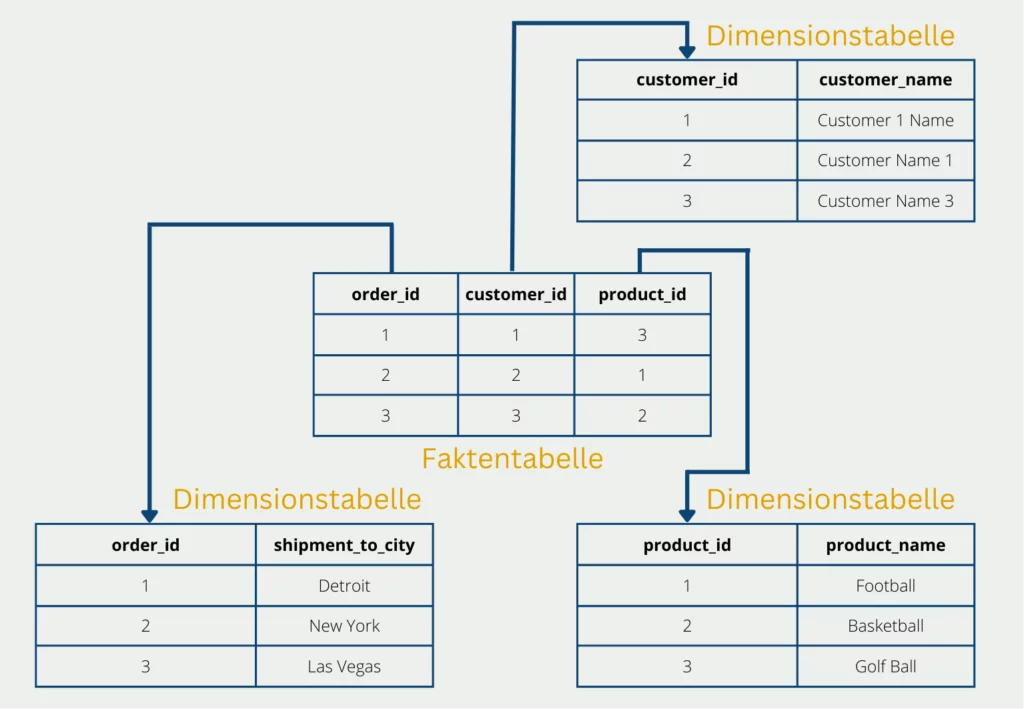
\includegraphics[scale=.25]{Bilder/SternSchemaDB.png}
\end{wrapfigure}

Der Primärschlüssel bezeichnet ein Attribut, das zur eindeutigen Identifikation einer Datenbankzeile verwendet werden kann. Dazu zählen beispielsweise die Rechnungsnummer zur Identifikation einer Rechnung oder die Ausweisnummer zur Identifikation einer Person.

\vspace{1em}

Konkret bedeutet dies in der Anwendung, dass \hl{alle Merkmale ausgelagert werden müssen, die nicht ausschließlich vom Primärschlüssel abhängig sind}. In der Praxis führt dies dann oft zu einem sogenannten Sternschema.


\paragraph{3. Normalform} Eine Relation liegt in der dritten Normalform vor, wenn sie in der ersten und zweiten Normalform vorliegt und \hl{keine transitiven Abhängigkeiten} bestehen.

Eine transitive Abhängigkeit liegt vor, wenn ein Attribut, welches kein Primärschlüssel ist, nicht nur von diesem abhängt, sondern auch von anderen Attributen.

Wenn wir in unserem Beispiel eine Tabelle haben, in der die Rechnungsnummer, die Produktnummer und der Preis gegeben ist, haben wir höchstwahrscheinlich eine transitive Abhängigkeit. \hl{Der Preis des Produktes hängt nämlich nicht wirklich von der Rechnungsnummer ab, sondern vielmehr von der Produktnummer}, da für jedes Produkt ein fester Preis definiert ist.

Diese Abhängigkeit kann man auflösen, indem man die Produkte in eine neue Tabelle auslagert und somit das Attribut Preis aus der ursprünglichen Tabelle rausfällt.

\subsubsection{Anomalien}
\label{sec:Anomalien}

Quelle: DatabaseCamp \cite{anomalien}

Anomalien in Datenbanken treten bei einer \hl{nicht existierenden oder fehlerhaften Normalisierung} auf.
Es existieren drei Arten von Datenbank-Anomalien, die Einfüge-Anomalie, die Änderungs-Anomalie und die Lösch-Anomalie.

In der Datenbanktentwicklung ist die Dritte Normalform oft ausreichend, um die perfekte Balance aus Redundanz, Performance und Flexibilität für eine Datenbank zu gewährleisten. Sie eliminiert auch die meisten Anomalien in einer Datenbank, aber nicht alle.

\paragraph{Einfügeanomalie} Bei einem fehlerhaften oder inkorrekten Datenbankdesign kann es bei der Einfüge-Anomalie passieren, dass Daten gar nicht in die Datenbank übernommen werden, wenn zum Beispiel der Primärschlüssel keinen Wert erhalten hat, oder eine \hl{unvollständigen Eingabe von Daten} zu Inkonsistenzen führt.

\paragraph{Änderungsanomalie} Bei der Änderungs-Anomalie, auch Update-Anomalie genannt, werden \hl{gleiche Attribute eines Datensatzes in einer Transaktion nicht automatisch geändert}. So entsteht eine Inkonsistenz der Daten.

\paragraph{Löschanomalie} Bei einer Löschanomalie kann es passieren, dass ein Benutzer einer Datenbank aktiv Informationen löschen will und damit indirekt, aufgrund des fehlerhaften Datenbankdesigns, \hl{andere zusammenhängende Informationen parallel mitlöscht}.